\chapter{ Origami Models: Simulations and Findings}

%Check for mail with subject "Energy diagrams for hexagonal cell"

\section{Deployable Origami Tubes}
Two types of triangulated Origami tubes were developed and were tested for deployability. In accordance with the idea of energy profile based on the sum of two angles of the triangular units of the tubes easy-deploy-easy-collapse and hard-deploy-hard-collapse tubes were developed\cite{Zha}. 

The cylindrical tube is generated by joining two edges of the sheet show in the Fig~\ref{fig:AlphaBeta}. For the angles shown in Fig~\ref{fig:AlphaBeta}, if $\alpha + \beta < 90^{\circ}$ the tube is of the easy-deploy-easy-collapse (Fig~\ref{fig:EDEC}) type and if the sum is greater than $90^{\circ}$ i.e $\alpha + \beta > 90^{\circ}$ the mechanism is of hard-deploy-hard-collapse type(Fig~\ref{fig:HDHC}). It was observed from analysis of numerical model that for the hard-deploy-hard-collapse model ($\alpha = 50^{\circ}, \beta = 50^{\circ}$), the strain in equivalent bar hinge model would be of the order 20\% and hence the collapse is not possible in normal paper model. Also the hard-deploy-hard-collapse model carried significant lode before the paper model underwent local buckling at its creases.
\begin{figure}[htbp]
\centering
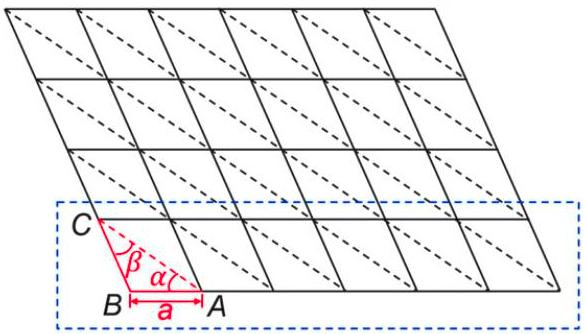
\includegraphics[width=0.6\linewidth]{Figures/AlphaBeta.jpg}
\caption{Crease Pattern For Cylindrical Tube}
\label{fig:AlphaBeta}
\end{figure}

\begin{figure}
\centering
\begin{minipage}{.5\textwidth}
  \centering
  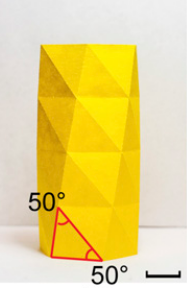
\includegraphics[width=.4\linewidth]{Figures/HardDeploy.png}
  \captionof{figure}{Hard-Deploy-Hard-Collapse}
  \label{fig:EDEC}
\end{minipage}%
\begin{minipage}{.5\textwidth}
  \centering
  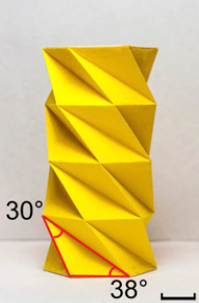
\includegraphics[width=.4\linewidth]{Figures/EasyDeploy.png}
  \captionof{figure}{Easy-Deploy-Easy-Collapse}
  \label{fig:HDHC}
\end{minipage}
\end{figure}


\section{Energy Profiles}
The simulated energy profiles for the origami tubes are shown in the Fig~\ref{fig:EnergyProfile}. The simulation was performed for the equivalent bar hinge model.
\begin{figure}[htbp]
\centering
	\subfigure[Easy-Collapse-Easy-deploy energy profile ]{
	\centering
		\label{fig:ECEDEP}
        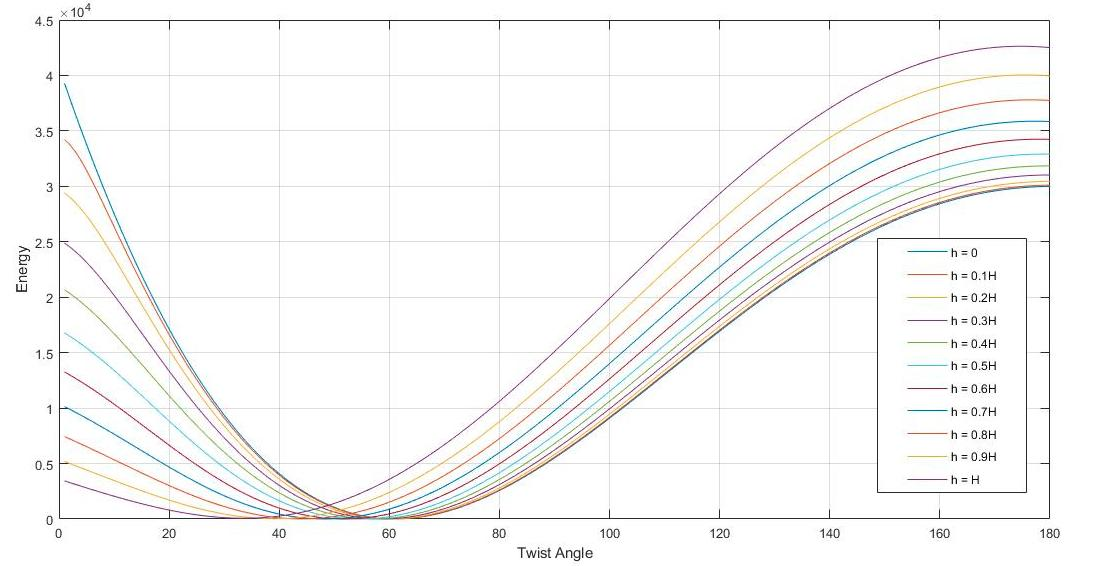
\includegraphics[width=1\linewidth]{Figures/EDEC.jpg}}
	\subfigure[Hard-Collapse-Hard-deploy energy profile]{
	\centering
		\label{fig:HCHDEP}
		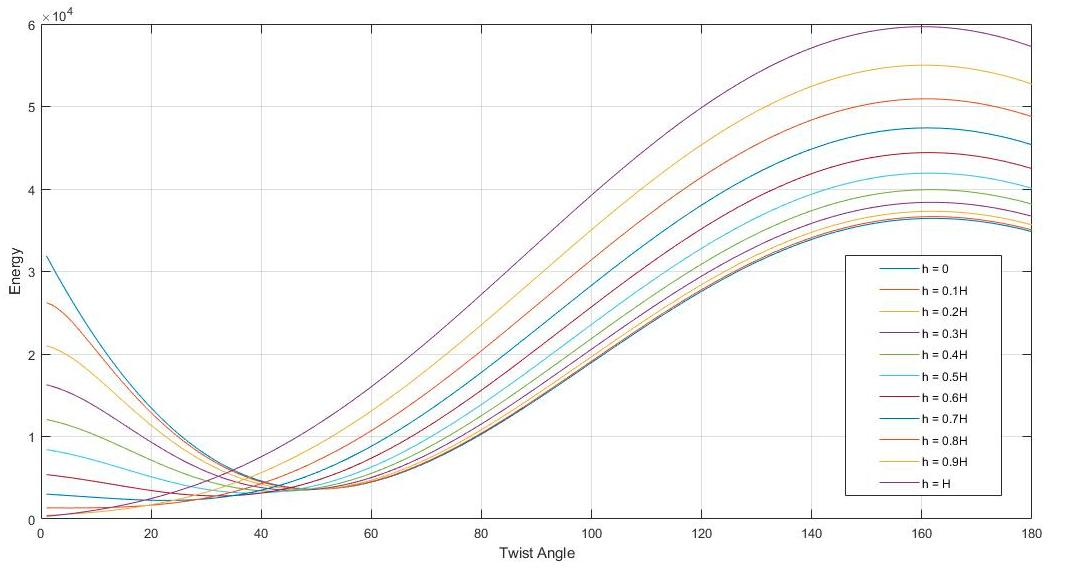
\includegraphics[width=1\linewidth]{Figures/HDHC.jpg}}
	\caption{Energy Profiles}
	\label{fig:EnergyProfile}
\end{figure}

As it can be seen from the energy profile obtained by computing energy in the structure at various stages of deployment, the easy-deploy-easy-collapse structure presents negligible energy barrier as opposed to the hard-deploy-hard-collapse structure in which significant energy barrier is present for process of deployment as well as collapse. 

Using metamaterials, a structure which presents no energy barrier during deployment but exhibits resistance to collapse can be developed. This will provide the reliability to the deployable structure without being dependent on locking mechanisms for its stability.

\section{Physical Models}
Physical models of the lattice were also developed to qualitatively validate the energy profiles obtained from simulation. The folding patterns used for the models are shown in the Fig~\ref{fig:HCHD_fold} and Fig~\ref{fig:ECED_fold}.
\begin{figure}[htbp]
    \centering
    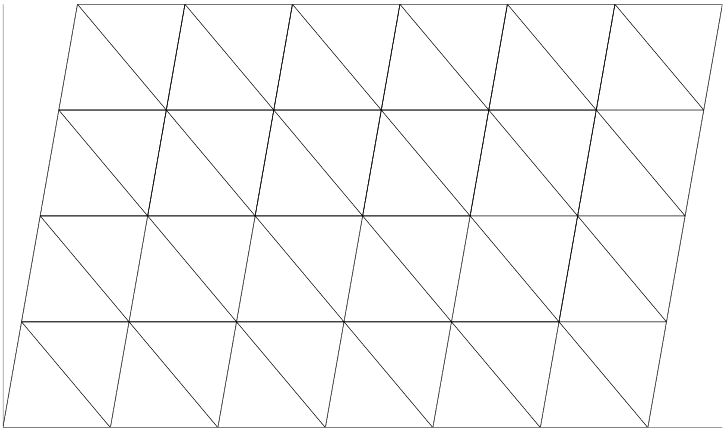
\includegraphics[width = 0.5\linewidth]{Figures/50_50_180_fold.png}
    \caption{Folding pattern for Hard-Collapse-Hard-Deploy Origami tube}
    \label{fig:HCHD_fold}
\end{figure}
\begin{figure}[htbp]
    \centering
    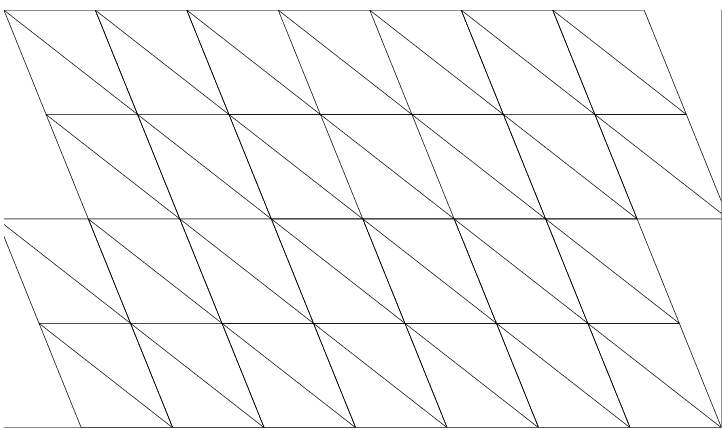
\includegraphics[width = 0.5\linewidth]{Figures/38_30_112_fold.png}
    \caption{Folding pattern for Easy-Collapse-Easy-Deploy Origami tube}
    \label{fig:ECED_fold}
\end{figure}

The models developed using these folding patterns are shown in the figures below. As predicted using the energy profiles, Easy-Deploy-Easy-Collapse type origami tube easily collapse under very small load from state shown in Fig~\ref{fig:EDEC_model} to the state shown in Fig~\ref{fig:EDEC_Model_Collapsed}. Also, the Hard-Deploy-Hard-Collapse (Fig~\ref{fig:HDHC_model}) type tube did not collapse in a way similar to Easy-Deploy-Easy-Collapse type tube even under high load (Fig~\ref{fig:HDHC_Model_Loaded}), but as stated earlier, due to developing high strains the paper began to tear and tube buckled.

\section{Conclusion}
From the models and simulation of origami tubes stated above we can conclude that modelling these origami tubes using bar hinge models and using metamaterials with different strengths in elongation and compression we can modify the energy profiles during deployment and collapse such that we have an selective Easy-Deploy-Hard-Collapse or Hard-Deploy-Easy-Collapse type structure.

\begin{figure}[htbp]
\centering
\begin{minipage}{.4\textwidth}
  \centering
  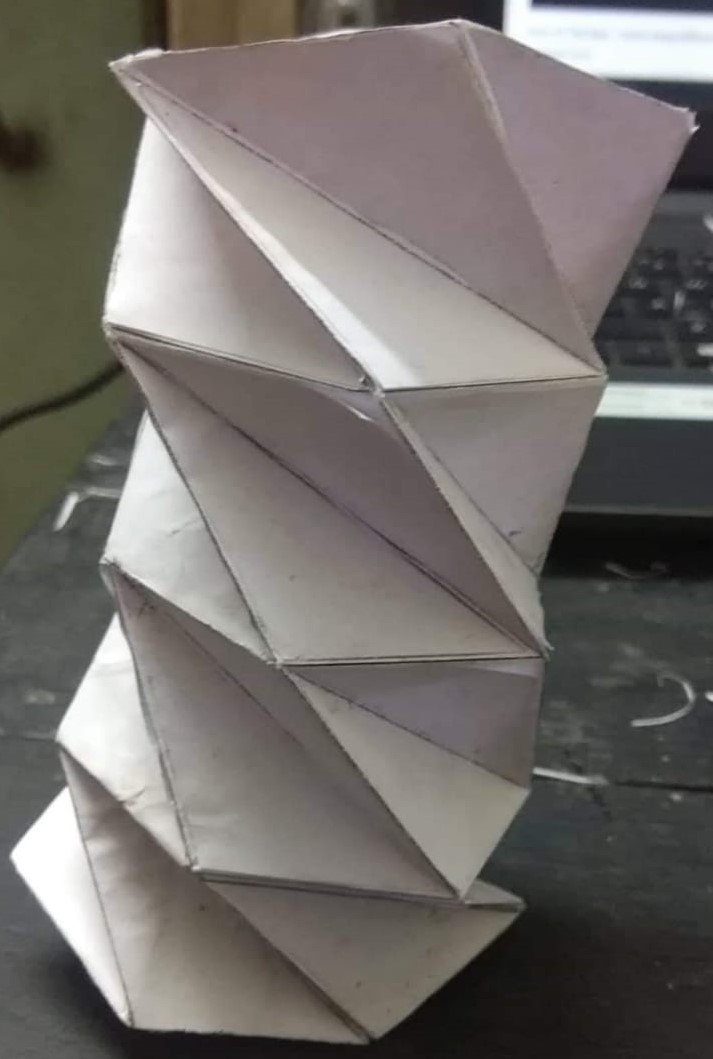
\includegraphics[width=.4\linewidth]{Figures/EDEC_Model.jpeg}
  \captionof{figure}{Easy-Deploy-Easy-Collapse physical model}
  \label{fig:EDEC_model}
\end{minipage}%
\hspace{2cm}
\begin{minipage}{.4\textwidth}
  \centering
  \vspace{2cm}
  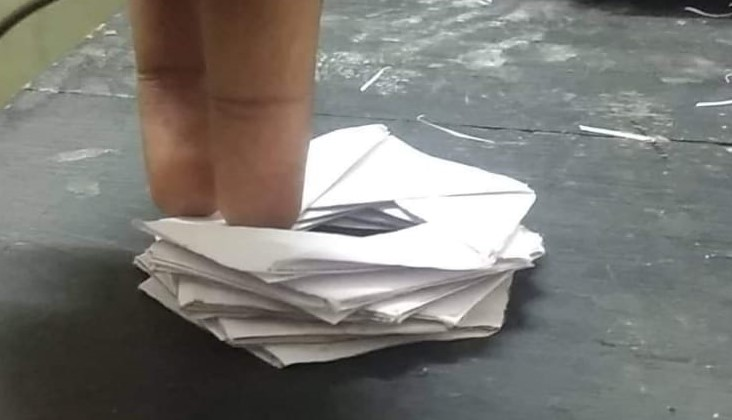
\includegraphics[width=.4\linewidth]{Figures/EDEC_Model_collapsed.jpeg}
  \captionof{figure}{Collapsed state of Easy-Deploy-Easy-Collapse Model}
  \label{fig:EDEC_Model_Collapsed}
\end{minipage}
\end{figure}
\vspace{-3cm}

\begin{figure}[htbp]
\centering
\begin{minipage}{.4\textwidth}
  \centering
  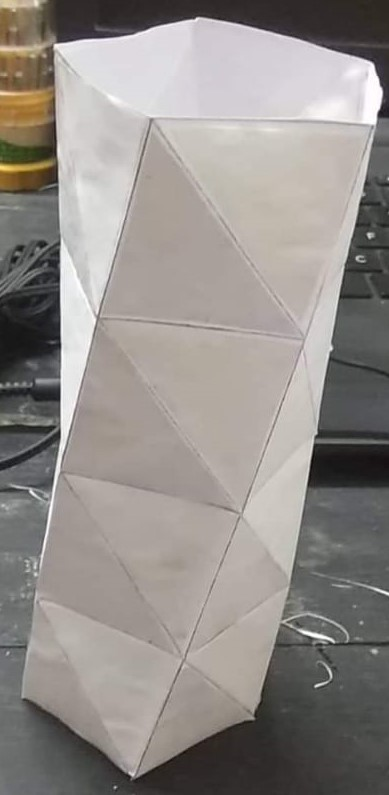
\includegraphics[width=.4\linewidth]{Figures/HDHC_Model.jpeg}
  \captionof{figure}{Hard-Deploy-Hard-Collapse physical model}
  \label{fig:HDHC_model}
\end{minipage}%
\hspace{2cm}
\begin{minipage}{.4\textwidth}
  \centering
  \vspace{0.4cm}
  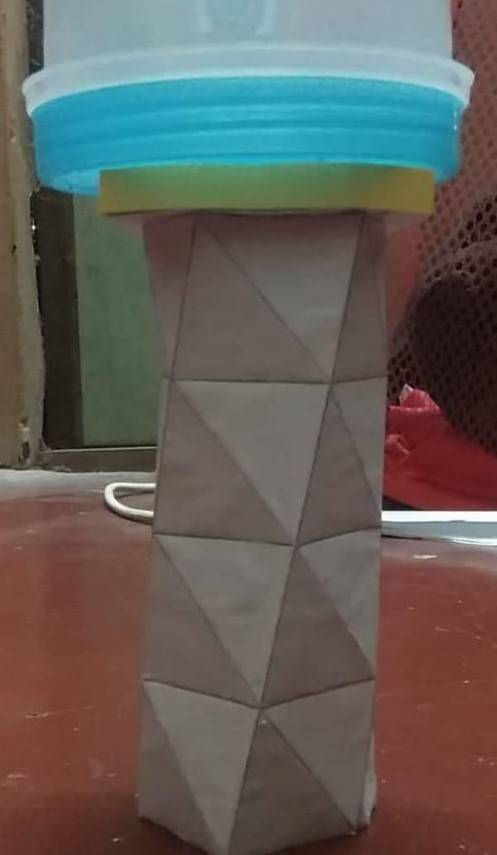
\includegraphics[width=.4\linewidth]{Figures/HDHC_Model_loaded.jpeg}
  \captionof{figure}{Hard-Deploy-Hard-Collapse Model under loading}
  \label{fig:HDHC_Model_Loaded}
\end{minipage}
\end{figure}